	\chapter{Sorteringsalgoritmer}
	\label{ch:Sorteringsalgoritmer}

	\section{Hvad er sortering?}
	\label{sec:Hvad er sortering?}



	Sortering er helt lavpraktisk at sætte en mængde data i rækkefølge på baggrund af disse datas attributter \cite{what-is-sorting}. Det kunne f.eks. være alfabetisk eller efter farve eller størrelse. Når man som menneske sorterer en hånd med kort er det ikke altid, at vi tænker over, hvordan vi gør. Det er dog ikke altid klart, hvilken sorterings-strategi, der vil være hurtigst. Disse sorterings-strategier kan også kaldes sorterings-algoritmer, og det er ikke kun mennesker, der kan benytte sorterings-algoritmer til f.eks. at sortere kort. Computere kan også, og de gør det for det meste også langt hurtigere. Resten af denne opgave omhandler to sorterings-algoritmer: insertionsort og mergesort, og deres forskellige måder at sortere en liste med tal.\\

	Herfra vil jeg kun forholde mig til sortering af lister med tal og sortere dem på baggrund af deres størrelse (se figur \ref{fig:Eksempel på sortering af en liste}). Derudover vil algoritmernes opgave altid være at sortere liste i stigende rækkefølge.

	\begin{figure}[h]
		\begin{center}
			$$[4,2,5,3,1] \:\:\longrightarrow\:\: [1,2,3,4,5]$$
		\end{center}
		\caption{Eksempel på sortering af en liste}
		\label{fig:Eksempel på sortering af en liste}
	\end{figure}


	\section{Insertionsort}
	\label{sec:Insertionsort}

	Insertionsort er en af de mere simple sorteringsalgoritmer. Pseudokoden til algoritmen kan ses i figur \ref{fig:Pseudokode til insertionsort} på side \pageref{fig:Pseudokode til insertionsort}. Koden er baseret på bogen \citetitle{aogd} \cite{aogd} s. 104.\\

	Det er ikke en tilfældighed, at denne algoritme hedder insertionsort. Den fungerer nemlig ved at gennemgå hvert element i listen og placere det, hvor det passer ind i de elementer, der allerede er sorterede. Dette er nok den måde, man ville sortere sin hånd i Uno eller 500. 


	\begin{figure}[h]
		\begin{center}
			\begin{lstlisting}
			funktion insertionsort(liste) {
				for i = 1 til i = n {					# her er n længden af listen
				e = liste[i]	 							# dette er elementet i listen

					if e < liste[0] {						# hvis elementet er større end det første element i listen
						for j = j til j = 0{ 
							liste[j] = liste[j-1]		# ryk elementerne på pladserne 0 til j et tak frem
						}
					liste[0] = e 							# sætter dette element forrest i listen
				}
				else{
					j = i 								# j er en nu tæller der starter på i
					while liste[j-1] > e {			# kør mens liste[j-1] er størren end elementet
						liste[j] = liste[j-1] 		# ryk liste[j] et tak til højre
						j -= 1
					}
					liste[j] = element				# indsæt elementet hvor det passer ind
				}
			}			
			return(liste)								# returnerer den sorterede liste
		}
		\end{lstlisting}
	\end{center}
	\vspace{-5mm}
	\caption{Pseudokode til insertionsort \cite[s. 104]{aogd}.}
	\label{fig:Pseudokode til insertionsort}
\end{figure}


	\subsection{Insertionsort Procedure}%
	\label{sub:Insertionsort Procedure}

	Vi kan allerede i linje 2 se, at algoritmen gennemgår alle elementerne i listen fra en ende af, da algoritmen her begynder med en for-løkke, der tæller for hvert element i listen, dog starter den ved 2. element i listen. For at gøre koden mere læsbar sættes elementet, som algoritmen er nået til, ind i variablen $e$ i linje 3. Det næste algoritmen gør, er at checke om elementet har en mindre værdi end det første element i listen. Hvis dette er sandt, rykkes alt før elementet et tak til højre, og elementet sættes ind først i listen (se figur \ref{fig:Indsæt element først i listen}). 

	% TODO computere rykker ikke!

	\begin{figure}[h]
		\begin{center}
			\padtable
			\begin{tabular}{l|c|c}
				Forklaring & Eksempel & Linje \\
				\hline
				Liste hvor \verb|e < liste[0]| & $[\blue{5},\blue{7},\blue{9},\red{4},6,5,2]$ & $5$ \\
				"Rykker" til højre & $[\blue{5},\blue{5},\blue{7},\blue{9},6,5,2]$ & $6$-$8$\\
				Sætter elementet ind først  & $[\red{4},\blue{5},\blue{7},\blue{9},6,5,2]$ & $9$
			\end{tabular}
		\end{center}
		\vspace{-3mm}
		\caption{Procedure for at indsætte element først i listen. Elementet er markeret med \red{rødt}, og tal der allerede er sorterede er markeret med \blue{blåt}. Linjer refererer til koden i figur \ref{fig:Pseudokode til insertionsort}.}
		\label{fig:Indsæt element først i listen}
	\end{figure}

	Det er vigtigt at pointere, at computere ikke kan "rykke"\ tal i en liste, men kun overskrive dem. Det er derfor at det ser ud som om at, computeren har dubleret $5$-tallet i figur \ref{fig:Indsæt element først i listen}. Det har den nemlig; den har taget de tre første elementer i listen, og skrevet dem over på andet, tredje og fjerde element. Computeren kan nu overskrive det første tal i listen, da det er en dublet.\\

	Vi er nu nået til linje $11$. Hvis ikke elementet er mindre end det første element i listen, sker følgende (se figur \ref{fig:Indsæt element hvor det passer i listen} på side \pageref{fig:Indsæt element hvor det passer i listen}): Algoritmen ser på tallet før elementet og spørger: "er dette tal større end elementet". Hvis det er, rykkes det til højre. Herefter stiller algoritmen samme spørgsmål til tallet \emph{to} pladser før elementet. Hvis dette tal er mindre and elementet, placerer algoritmen elementet efter dette tal i listen, hvis ikke stiller den samme spørgsmål til tallet 3 pladser før elementet og så videre. Det er vigtigt at pointere, at der altid vil være et tal, der er mindre end elementet, da elementet ellers ville være blevet placeret først i listen af den første del af proceduren (linje $5$-$10$).


	\begin{figure}[h]
		\begin{center}
		\padtable
		\begin{tabular}{l|c|c}
			Forklaring & Eksempel & Linje\\
			\hline
			Liste hvor \verb|e >= liste[0]| & $[\blue{4},\blue{5},\blue{7},\blue{9},\red{6},5,2]$ &$11$\\
			Da $9 \geq 6$ rykkes tallet til højre & $[\blue{4},\blue{5},\blue{7},\blue{9},\blue{9},5,2]$ & $13$-$14$\\
			Da $7 \geq 6$ rykkes tallet til højre & $[\blue{4},\blue{5},\blue{7},\blue{7},\blue{9},5,2]$ & $13$-$14$\\
			Da $5 \ngeq 6$ sættes elementet ind efter $5$ & $[\blue{4},\blue{5},\red{6},\blue{7},\blue{9},5,2]$ & $13$ og $17$
		\end{tabular}
	\end{center}
	\vspace{-3mm}
	\caption{Procedure for at indsætte et element hvor det passer i den sorterede liste. Elementet er markeret med \red{rødt}, og tal der allerede er sorterede er markeret med \blue{blåt}. Linjer refererer til figur \ref{fig:Pseudokode til insertionsort}.}
	\label{fig:Indsæt element hvor det passer i listen}
\end{figure}



\subsection{Egenskaber af Insertionsort}%
\label{sub:Egenskaber af Insertionsort}
Insertionsort er en god sorteringsalgoritme, idet proceduren er forholdsvis nem at forstå, og fordi listen til venstre for det element algoritmen er nået til ($e$), altid vil være sorteret. Hvis man stopper en insertionsort-algoritme halvvejs gennem dens køretid, vil man altid have en liste, hvor den første halvdel er sorteret og den anden halvdel usorteret. Denne egenskab har mergesort ikke.\\

Se afsnit \ref{sec:Analyse af Insertionsort} for store-O analysen af insertionsort.



\section{Mergesort}
\label{sec:Mergesort}

Hvor insertionsort er en løkke-baseret algoritme, er mergesort rekursiv, idet den ikke benytter en løkke til at gentage instruktioner, men kalder sig selv i stedet. Dette leder til en fraktallignende sorteringsmetode, der deler problemet i mindre og mindre bidder. 

\subsection{Mergesort Procedure}%
\label{sub:Mergesort Procedure}

Pseudokoden til denne algoritme kan findes i figur \ref{fig:Pseudokode til mergesort} på side \pageref{fig:Pseudokode til mergesort}. Koden er basseret på kilde \cite[s. 106]{aogd}.\\

Mergesortalgoritmen består af to funktioner. Lad os begynde med funktionen $merge$, da det er den mest simple. Koden til funktionen kan findes på figur \ref{fig:Pseudokode til mergesort} linje $11$-$29$. Funktionen tager to lister ($a$ og $b$) som argumenter, og fletter dem sammen til en tredje liste ($c$) (se figur \ref{fig:merge i mergesort}). Denne $c$ liste er dog ikke nødvendigvis sorteret. Eksempelvis kunne dette være en returneret liste:

$$merge([1,2,4,8],[9,5,6,4,7]) \longrightarrow [\orange{1}, \orange{2}, \orange{4}, \orange{8}, \orange{9}, \blue{5}, \blue{6}, \violet{4}, \violet{7}]$$

Her er resultatet en delvist sorteret liste bestående af flere sorterede dele. Altså kan vi ikke nøjes med $merge$ for at sortere en liste. En vigtig egenskab af $merge$ er dog, at den kan flette to sorterede lister sammen til én samlet sorteret liste. Det kunne for eksempel være i dette tilfælde:

$$merge([1,3,4,8],[2,3,6,7,7]) \longrightarrow [1, 2, 3, 3, 4, 6, 7, 7, 8]$$

Her er begge argumenter ($a$ og $b$) sorterede lister, der flettes sammen til én samlet sorteret liste.\\


\begin{figure}
\begin{center}
	\begin{lstlisting}
		funktion mergesort(liste) {
			if liste.length == 1{ 		# hvis listen har en længde på 1: returner listen uændret
				return(liste)
			}
			else {
				# Her deler algoritmen først listen i to dele. Derefter kalder den sig selv på hver del. Dette gør den til listerne kun er indeholder et element. Derefter samles dellisterne til en samlet og sorteret liste af mergefunktionen
				return(merge(mergesort(liste[0 ... n/2]), mergesort(liste[n/2 + 1 ... n])))
			}
		}

		funktion merge(a,b) {
			c = []							# Listen a og b flettes ind i

			while(true) {					# Lykken kører til der returneres en værdi 
				if a.length == 0 {		# Hvis der ikke er mere i a
					return(c + b)			# Returnerer c sammenføjet med b
				}
				elif b.length == 0 {		# Ellers hvis der ikke er mere i b
					return(c + a)			# Returnerer c sammenføjet med a
				}
				elif a[0] <= b[0] {		# Ellers hvis det første element i a er mindre end det i b
					tilføj a[0] til c
					fjern a[0] fra a
				}
				else {						# Ellers
					tilføj b[0] til c
					fjern b[0] fra b
				}
			}
		}

	\end{lstlisting}
\end{center}
\vspace{-5mm}
\caption{Pseudokode til Mergesort \cite[s. 106]{aogd}.}
\label{fig:Pseudokode til mergesort}
\end{figure}



\begin{figure}
\begin{center}
	\padtable
	\begin{tabular}{l|c|c|c|c}
		Forklaring & $a$ & $b$ & $c$ & Linje\\
		\hline
		 Da $a[0] \leq b[0]$ føjes $a[0]$ til $c$ & $[\red{3},6,6]$ & $[\red{4},5,7,9]$ & [\:] & $18$-$21$\\
		 Da $a[0] \nleq b[0]$ føjes $b[0]$ til $c$ & $[\red{6},6]$ & $[\red{4},5,7,9]$ & $[\violet{3}]$ & $22$-$25$\\
		 Da $a[0] \nleq b[0]$ føjes $b[0]$ til $c$ & $[\red{6},6]$ & $[\red{5},7,9]$ & $[\blue{3},\violet{4}]$ & $22$-$25$\\
		 Da $a[0] \leq b[0]$ føjes $a[0]$ til $c$ & $[\red{6},6]$ & $[\red{7},9]$ & $[\blue{3},\blue{4},\violet{5}]$ & $18$-$21$\\
		 Da $a[0] \leq b[0]$ føjes $a[0]$ til $c$ & $[\red{6}]$ & $[\red{7},9]$ & $[\blue{3},\blue{4},\blue{5},\violet{6}]$ & $18$-$21$\\
		 Da $a.length = 0$ føjes $b$ til $c$ & $\red{[\:]}$ & $[7,9]$ & $[\blue{3},\blue{4},\blue{5},\blue{6},\violet{6}]$ & $12$-$14$\\
		 Returnerer $c$ & $[\:]$ & $[\:]$ & $[\blue{4},\blue{5},\blue{3},\blue{6},\blue{1},\violet{7},\violet{9}]$ & $13$\\
	\end{tabular}
\end{center}
\caption{Eksempel med delfunktionen \emph{merge} i mergesort. Her kalder vi merge($[3,6,6]$, $[4,5,7,9]$). I hvert trin sammenlignes de \red{røde } tal. \blue{Blå }tal er en del af den færdige $c$ liste, og \violet{lilla } tal er de tal der sidst blev føjet til $c$. Læg mærke til at den endelige $c$ liste er sorteret fordi listerne $a$ og $b$ på forhånd var sorterede. Linjer refererer til figur \ref{fig:Pseudokode til mergesort}.}
\label{fig:merge i mergesort}
\end{figure}

Linjenumre i det næste afsnit refererer til pseudokoden til algoritmen på figur \ref{fig:Pseudokode til mergesort} på side \pageref{fig:Pseudokode til mergesort}.\\

Mergesorts kompleksitet kommer dog først rigtigt til udtryk, når vi tager hele algoritmen i betragtning. Mergesortfunktionen (l. $1$) tager en enkel liste som argument og checker først, om listen kun indeholder ét element (l. $2$). Hvis den gør, så returnerer den listen uændret (l. $3$). Dette giver intuitivt mening, da en liste med et enkelt element altid vil være sorteret. Hvis listen er \emph{mere} end $1$ lang, gør den det, som får hele algoritmen til at fungere (l. $5$-$8$): den deler listen i to, og kalder sig selv på hver halvdel. Herefter sættes de to dele sammen igen af $merge$-funktionen. Det er dog ikke helt så enkelt, som det lyder, idet $mergesort$ rekursivt kalder sig selv. Det leder til, at algoritmen splitter listen op igen og igen, indtil der kun er et element i de mange lister. Herefter samler $merge$ alle de små lister til en stor liste, hvor $merge$ løbende sørger for, at de lister den samler er sorterede (se figur \ref{fig:mergesort_procedure}). De lister, der er samlet af $merge$, vil altid være sorterede, da udgangspunktet er lister med et enkelt element. Disse enkelt-element-lister samles af $merge$ til lister med to elementer der er sorterede. Og disse sorterede lister sættes sammen med andre sorterede lister. $merge$ får altid to sorterede lister som input, og spytter derfor altid en samlet sorteret liste ud som output.


  \small
\begin{minipage}{0.4\textwidth}
  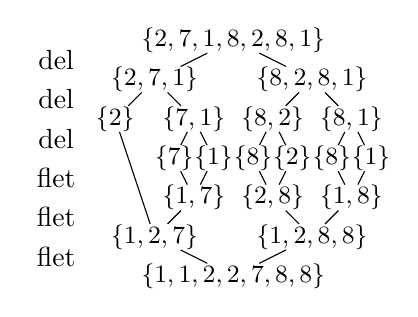
\begin{tikzpicture}[scale =.5,
    s/.style = {font = \small, inner sep = 0pt}]
    \node (2718281) at (-.5,0)  [s] {$\{2,7,1,8,2,8,1\}$};
    \node (1122788) at (-.5,-6) [s] {$\{1,1,2,2,7,8,8\}$};
    \node (271)     at (-2.5,-1)[s] {$\{2,7,1\}$};
    \node (127)     at (-2.5,-5)[s] {$\{1,2,7\}$};
    \node (2)       at (1,-3)   [s] {$\{2\}$};
    \node (2u)      at (-3.5,-2)[s] {$\{2\}$};
    \node (71)      at (-1.5,-2)[s] {$\{7,1\}$};
    \node (17)      at (-1.5,-4)[s] {$\{1,7\}$};
    \node (7)       at (-2,-3)  [s] {$\{7\}$};
    \node (8281)    at (1.5,-1) [s] {$\{8,2,8,1\}$};
    \node (1288)    at (1.5,-5) [s] {$\{1,2,8,8\}$};
    \node (81)      at (2.5,-2) [s] {$\{8,1\}$};
    \node (18)      at (2.5,-4) [s] {$\{1,8\}$};
    \node (1a)       at (-1,-3) [s] {$\{1\}$};
    \node (1b)       at (3,-3)  [s] {$\{1\}$};
    \node (8a)      at (0, -3)  [s] {$\{8\}$};
    \node (8b)      at (2,-3)   [s] {$\{8\}$};
    \node (82)      at (0.5,-2) [s] {$\{8,2\}$};
    \node (28)      at (0.5,-4) [s] {$\{2,8\}$};
    \node at (-5,-0.5) {del};
    \node at (-5,-1.5) {del};
    \node at (-5,-2.5) {del};
    \node at (-5,-3.5) {flet};
    \node at (-5,-4.5) {flet};
    \node at (-5,-5.5) {flet};
    \draw  (2718281) -- (271);
    \draw  (2718281) -- (8281);
    \draw  (271) -- (2u);
    \draw  (271) -- (71);
    \draw  (8281) -- (82);
    \draw  (8281) -- (81);
    \draw  (71) -- (7);
    \draw  (71) -- (1a);
    \draw  (82) -- (8a);
    \draw  (82) -- (2);
    \draw  (81) -- (8b);
    \draw  (81) -- (1b);
    \draw  (8a) -- (28);
    \draw  (2) -- (28);
    \draw  (7) -- (17);
    \draw  (1a) -- (17);
    \draw  (8b) -- (18);
    \draw  (1b) -- (18);
    \draw  (2u) -- (127);
    \draw  (17) -- (127);
    \draw  (28) -- (1288);
    \draw  (18) -- (1288);
    \draw  (127) -- (1122788);
    \draw  (1288) -- (1122788);
  \end{tikzpicture}
\end{minipage}
\begin{minipage}{0.55\textwidth}
\begin{flushright}%
\begin{tabular}{rrl|l}
$a$ & $b$ & $c$ & Operation\\
\hline
$\{1,2,7\}$ &$ \{1,2,8,8\}$ &  $ \{\,\}$ & flyt fra $a$\\
$\{2,7\}$ &$ \{1,2,8,8\}$ &  $ \{1\}$ & flyt fra $b$\\
$\{2,7\}$ &$ \{2,8,8\}$ &  $ \{1,1\}$ & flyt fra $a$\\
$\{7\}$ &$ \{2,8,8\}$ &  $ \{1,1,2\}$ & flyt fra $b$\\
$\{7\}$ &$ \{8,8\}$ &  $ \{1,1,2,2\}$ & flyt fra $a$\\
$\{\,\}$ &$ \{8,8\}$ &  $ \{1,1,2,2,7\}$ & sammenføj $b$\\
$\{\,\}$ &$ \{\,\}$ &  $ \{1,1,2,2,7,8,8\}$ & \\
\end{tabular}
\end{flushright}
\end{minipage}



\subsection{Tidskompleksiteten af Mergesort}
\label{sec:Tidskompleksiteten af Mergesort}

Mergesort har tidskompleksiteten $O(n \cdot \log n)$ \cite{big-o-cheatsheet}. Algoritmens værste-tilfælde-vækstrate er det samme som vækstraten af $n \cdot \log n$.

$$T_{\text{mergesort}} \in O(n \cdot \log n)$$


\section{Store-O-Analyse af Insertionsort}
\label{sec:Analyse af Insertionsort}

I dette afsnit gøres der brug af tidligere definerede begreber og koncepter fra afsnit \ref{ch:Algoritmers Udførelsestid}.

\subsection{Insertionsort i Værste Tilfælde}%
\label{sub:Insertionsort i Værste Tilfælde}


Når man analyserer en algoritme teoretisk handler det ikke om den faktiske udførelsestid, men nærmere hvor mange operationer computeren skal køre for at fuldføre algoritmen. På den måde kan man abstrahere helt væk fra fysisk tid og regne med teoretiske operationer, hvis reelle udførelsestid ikke har nogen indflydelse. Det er fordi udførelsestiden er proportional med antallet af operationer, der kører på computerens cpu. Den eneste faktor for antallet af operationer, som en sorteringsalgoritme kører, er kardinaliteten af inputtet algoritmen udføres på. Dette gør det muligt at beskrive antallet af operationer (der er propportionalt med udførelsestiden) udelukkende som funktion af $n$ (inputtets kardinalitet). \cite[s. 42]{aogd}\\


Insertionsort består af to løkker: en indre og en ydre. Den ydre løkke kører fra $i = 1$ til (og uden) $i = n$. Altså kører koden inde i løkken $n - 1$ gange. Den indre løkke kører i værste tilfælde fra $j = i$ til $j = 1$ for hver $i$ værdi i den ydre løkke. Det betyder, at operationerne, som den indre løkke udfører, stiger sammen med $i$ (se figur \ref{fig:Insertionsort Operationer i løkker} på side \pageref{fig:Insertionsort Operationer i løkker}). Vi ender med at kunne beskrive det totale antal gange som koden i den indre løkke kører, som summen af alle $i$-værdierne, som den ydre løkke gennemgår. Koden i den indre lykke køres $i-1$ gange for hver $i$.

$$\sum_{i=2}^{n}i-1$$

Den indre løkkes kode køres $i$ gange, da løkken gennemgår fra $j=i$ til og med $j=1$, altså kører løkken $i$ gange. Vi kan nu omskrive summen således:

$$\sum_{i=1}^{n-1}i$$

For at simplificere udtrykket endnu mere kan vi bruge reglen at en sum som $1 + \dots + n -1$ kan omskrives på denne måde. 

$$\sum_{i=1}^{n-1}i \s=\s \frac{n(n-1)}{2} \s=\s \frac{1}{2}\cdot  n^2 - \frac{1}{2}\cdot  n$$

Dette er altså et udtryk for, hvor mange gange koden i den indre løkke kører som funktion af kardinaliteten af algoritmens input. Vi kunne nu begynde at gange denne funktion med hvor mange operationer, der sker inde i den indre løkke. Og lægge operationerne der sker $n$ gange til, fordi de er med i den ydre løkke. Til sidst kunne vi lægge de operationer, der kun sker én gang til, og resultatet ville se nogenlunde sådan ud:

$$a \cdot \frac{1}{2} \cdot n^2 - a \cdot \frac{1}{2} \cdot n + b \cdot n + c$$

Her er $a$ antallet af operationer i den indre løkke, $b$ er antallet af operationer kun i den ydre løkke, og $c$ er operationerne, som er uden for begge løkker. Det smarte ved store-O-notation er at vi faktisk ikke behøver at kende de reelle værdier for $a$, $b$ og $c$, da de alle er konstanter, og derfor ikke har nogen indflydelse på algoritmens vækstrate. Selv ikke udførelsestiden for hver at disse operationer har nogen indflydelse på vækstraten. Vi kan derfor sige, at algoritmens udførelsestid er $O(n^2)$.

$$T_{\text{insertionsort}}(n) \in O(n^2)$$

Med det menes, at udførelsestiden i værste tilfælde har tidskompleksiteten $\Theta (n^2)$.


\begin{figure}[b]
	\begin{center}
		\padtable
		\begin{tabular}{ c|c|c }
			i & j & kørsler i $j$ løkken\\
			\hline
			$2$ & $2 \dots 1$ & $1$\\
			$3$ & $3 \dots 1$ & $2$\\
			$4$ & $4 \dots 1$ & $3$\\
			$5$ & $5 \dots 1$ & $4$\\
			\vdots & \vdots & \vdots\\
			$n$ & $n \dots 1$ & $(n-1)$\\
		\end{tabular}
		$\s\s \Longrightarrow \s\s $	
		\begin{tabular}{c}
			Total antal kørsler i $j$-løkken:\\
			%\hline
			\vspace{-4mm}
			\\
			$\displaystyle\sum_{i=1}^{n-1}i=\frac{n(n-1)}{2}$
		\end{tabular}
	\end{center}
	\caption{Insertionsort: Antal kørsler af koden i den indre $j$-løkke, hvis inputlisten har kardinaliteten $n$}
	\label{fig:Insertionsort Operationer i løkker}
\end{figure}


